\documentclass[a4paper,10pt]{article}

\usepackage[ansinew]{inputenc}
\usepackage[spanish]{babel}
\usepackage{graphicx}
\usepackage{listings}
\usepackage{appendix}
\usepackage{pdfpages}
\usepackage{fancyhdr}
\usepackage{ulem}
\pagestyle{fancy}

\def\dashuline{\bgroup 
  \ifdim\ULdepth=\maxdimen  % Set depth based on font, if not set already
   \settodepth\ULdepth{(j}\advance\ULdepth.4pt\fi
  \markoverwith{\kern.15em
  \vtop{\kern\ULdepth \hrule width .3em}%
  \kern.15em}\ULon}

\begin{document}

\lhead{\fancyplain{}{Base de Datos 75.15}}
\rhead{\fancyplain{}{Trabajo Pr\'actico Grupal}}

\setcounter{page}{2}

\newpage
\thispagestyle{empty}
\tableofcontents

\newpage
\section{Modelo Entidad Relaci\'on}
  \subsection{Diagrama}
    \begin{center}
      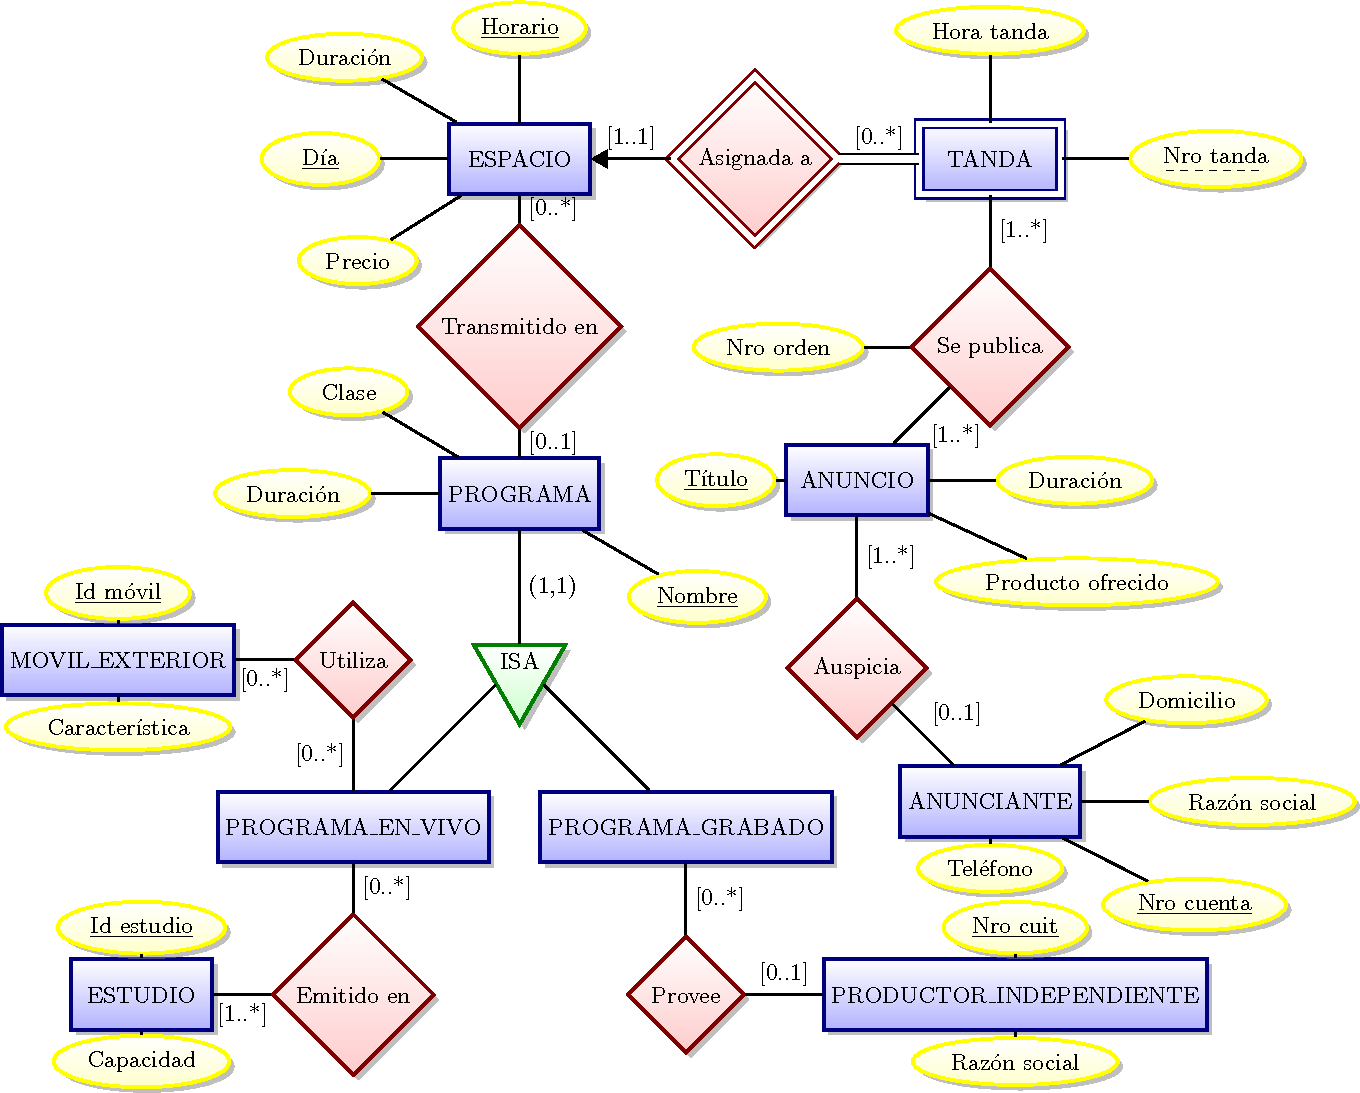
\includegraphics[width=18cm, height=12cm, angle=-90]{ModeloE-R/ModeloE-R.png}   
    \end{center}
  \subsection{Hip\'otesis}
    \begin{enumerate}
      \item Cada m\'ovil de exterior posee un id que lo identifica un\'ivocamente. 
      \item Un programa puede ser en vivo o grabado.
      \item S\'olo los programas en vivo poseen estudios de emisi\'on.
    \end{enumerate}
    
  \subsection{Diccionario}
    \subsubsection{Entidades}
    \begin{flushleft}
      \begin{large} \bf{Espacio} \end{large}
    \end{flushleft}
      \begin{tabular}{| p{2cm} | p{9cm} |}
	\hline
	\multicolumn{2}{|l|}{\bf{Descripci\'on:}} \\
	\hline
	\multicolumn{2}{|l|}{Un espacio es una divisi\'on del horario de transmisi\'on del canal.} \\
	\hline	
	\multicolumn{2}{|l|}{\bf{Especificaci\'on de atributos:}} \\
	\hline
	- D\'ia & El d\'ia en el que se emite el espacio. \\
	\hline \hline
	- Horario & El horario en el que se emite el espacio. \\
	\hline \hline
	- Duraci\'on & La duraci\'on del espacio.\\
	\hline \hline
	- Precio & El precio por segundo en el aire del espacio.\\
	\hline
	\multicolumn{2}{|l|}{\bf{Especificaci\'on de identificador \'unico:}} \\
	\hline
	\multicolumn{2}{|l|}{- D\'ia + Horario} \\
	\hline
      \end{tabular}
    
    \begin{flushleft}
      \begin{large} \bf{Tanda} \end{large}
    \end{flushleft}
      \begin{tabular}{| p{2cm} | p{9cm} |}
	\hline
	\multicolumn{2}{|l|}{\bf{Descripci\'on:}} \\
	\hline
	\multicolumn{2}{|l|}{Un tanda es un espacio donde se publicitan anuncios.} \\
	\hline	
	\multicolumn{2}{|l|}{\bf{Especificaci\'on de atributos:}} \\
	\hline
	- Hora tanda & La hora de comienzo de la tanda. \\
	\hline \hline
	- Nro tanda & El n\'umero de tanda correspondiente a un programa. \\
	\hline
	\multicolumn{2}{|l|}{\bf{Especificaci\'on de identificador \'unico:}} \\
	\hline
	\multicolumn{2}{|l|}{- D\'ia + Hora tanda + Nro tanda} \\
	\hline
      \end{tabular}

    \begin{flushleft}
      \begin{large} \bf{Anuncio} \end{large}
    \end{flushleft}
      \begin{tabular}{| p{2cm} | p{9cm} |}
	\hline
	\multicolumn{2}{|l|}{\bf{Descripci\'on:}} \\
	\hline
	\multicolumn{2}{|l|}{Un anuncio es un espacio, dentro de una tanda, destinado a dar a conocer} \\
	\multicolumn{2}{|l|}{un producto.} \\
	\hline	
	\hline	
	\multicolumn{2}{|l|}{\bf{Especificaci\'on de atributos:}} \\
	\hline
	- T\'itulo & El t\'itulo del anuncio. \\
	\hline \hline
	- Duraci\'on & La duraci\'on del anuncio. \\
	\hline \hline
	- Producto \newline ofrecido & El producto ofrendido del anuncio. \\
	\hline
	\multicolumn{2}{|l|}{\bf{Especificaci\'on de identificador \'unico:}} \\
	\hline
	\multicolumn{2}{|l|}{- T\'itulo} \\
	\hline
      \end{tabular}

    \begin{flushleft}
      \begin{large} \bf{Anunciante} \end{large}
    \end{flushleft}
      \begin{tabular}{| p{2cm} | p{9cm} |}
	\hline
	\multicolumn{2}{|l|}{\bf{Descripci\'on:}} \\
	\hline
	\multicolumn{2}{|l|}{Un anunciante auspicia a lo sumo un producto, mediante un anuncio.} \\
	\hline	
	\multicolumn{2}{|l|}{\bf{Especificaci\'on de atributos:}} \\
	\hline
	- Nro cuenta & El n\'umero de cuenta del anunciante. \\
	\hline \hline
	- Domicilio & El domicilio del anunciante. \\
	\hline \hline
	- Raz\'on \newline social & La raz\'on social del anunciante. \\
	\hline \hline
	- Tel\'efono & El tel\'efono del anunciate. \\
	\hline
	\multicolumn{2}{|l|}{\bf{Especificaci\'on de identificador \'unico:}} \\
	\hline
	\multicolumn{2}{|l|}{- Nro cuenta} \\
	\hline
      \end{tabular}
  \begin{flushleft}
      \begin{large} \bf{Programa} \end{large}
    \end{flushleft}
      \begin{tabular}{| p{2cm} | p{9cm} |}
	\hline
	\multicolumn{2}{|l|}{\bf{Descripci\'on:}} \\
	\hline
	\multicolumn{2}{|l|}{Un programa es un bloque con contenido que transmitir\'a el canal periodicamente} \\
	\hline	
	\multicolumn{2}{|l|}{\bf{Especificaci\'on de atributos:}} \\
	\hline
	- Clase & El tipo de programa que se transmite. \\
	\hline \hline
	- Nombre & Nombre del programa. \\
	\hline \hline
	- Duraci\'on & La duraci\'on del programa.\\
	\hline
	\multicolumn{2}{|l|}{\bf{Especificaci\'on de identificador \'unico:}} \\
	\hline
	\multicolumn{2}{|l|}{- Nombre} \\
	\hline
      \end{tabular}
  
  \begin{flushleft}
      \begin{large} \bf{Programa en vivo} \end{large}
    \end{flushleft}
      \begin{tabular}{| p{2cm} | p{9cm} |}
	\hline
	\multicolumn{2}{|l|}{\bf{Descripci\'on:}} \\
	\hline
	\multicolumn{2}{|l|}{Un programa en vivo es un programa que se transmite en vivo} \\
	\hline	
	\multicolumn{2}{|l|}{\bf{Especificaci\'on de atributos:}} \\
	\hline
	- No tiene & \\
	\hline
	\multicolumn{2}{|l|}{\bf{Especificaci\'on de identificador \'unico:}} \\
	\hline
	\multicolumn{2}{|l|}{- Hereda la clave de la entidad Programa} \\
	\hline
      \end{tabular} 
  
  \begin{flushleft}
      \begin{large} \bf{Programa grabado} \end{large}
    \end{flushleft}
      \begin{tabular}{| p{2cm} | p{9cm} |}
	\hline
	\multicolumn{2}{|l|}{\bf{Descripci\'on:}} \\
	\hline
	\multicolumn{2}{|l|}{Un programa grabado es un programa que se graba y luego se transmite} \\
	\hline	
	\multicolumn{2}{|l|}{\bf{Especificaci\'on de atributos:}} \\
	\hline
	- No tiene & \\
	\hline
	\multicolumn{2}{|l|}{\bf{Especificaci\'on de identificador \'unico:}} \\
	\hline
	\multicolumn{2}{|l|}{- Hereda la clave de la entidad Programa} \\
	\hline
      \end{tabular}
      
  	
  	\begin{flushleft}
      \begin{large} \bf{Movil Exterior} \end{large}
    \end{flushleft}
      \begin{tabular}{| p{2cm} | p{9cm} |}
	\hline
	\multicolumn{2}{|l|}{\bf{Descripci\'on:}} \\
	\hline
	\multicolumn{2}{|l|}{Un movil exterior es un veh\'iculo preparado para usar en la calle durante la emisi\'on de programas en vivo} \\
	\hline	
	\multicolumn{2}{|l|}{\bf{Especificaci\'on de atributos:}} \\
	\hline
	- IdMovil & Identifica el movil. \\
	\hline \hline
	- Caracter\'istica & Descripci\'on de las caracter\'isticas del movil. \\
	\hline
	\multicolumn{2}{|l|}{\bf{Especificaci\'on de identificador \'unico:}} \\
	\hline
	\multicolumn{2}{|l|}{- IdMovil} \\
	\hline
      \end{tabular}
      
     	\begin{flushleft}
      \begin{large} \bf{Estudio} \end{large}
    \end{flushleft}
      \begin{tabular}{| p{2cm} | p{9cm} |}
	\hline
	\multicolumn{2}{|l|}{\bf{Descripci\'on:}} \\
	\hline
	\multicolumn{2}{|l|}{Un estudio es el lugar donde se toma lugar un programa en vivo} \\
	\hline	
	\multicolumn{2}{|l|}{\bf{Especificaci\'on de atributos:}} \\
	\hline
	- IdEstudio & Identifica el estudio. \\
	\hline \hline
	- Capacidad & Cantidad de personas que entran en el estudio. \\
	\hline
	\multicolumn{2}{|l|}{\bf{Especificaci\'on de identificador \'unico:}} \\
	\hline
	\multicolumn{2}{|l|}{- IdEstudio} \\
	\hline
      \end{tabular} 
      
      \begin{flushleft}
      \begin{large} \bf{Productor independiente} \end{large}
    \end{flushleft}
      \begin{tabular}{| p{3cm} | p{9cm} |}
	\hline
	\multicolumn{2}{|l|}{\bf{Descripci\'on:}} \\
	\hline
	\multicolumn{2}{|l|}{Un productor independiente es aquel que se graba un programa y lo entrega al canal para ser transmitido} \\
	\hline	
	\multicolumn{2}{|l|}{\bf{Especificaci\'on de atributos:}} \\
	\hline
	- NroCuit & N\'umero de CUIT del productor. \\
	\hline \hline
	- Raz\'on \newline Social & Raz\'on social del productor\\
	\hline
	\multicolumn{2}{|l|}{\bf{Especificaci\'on de identificador \'unico:}} \\
	\hline
	\multicolumn{2}{|l|}{- NroCuit} \\
	\hline
      \end{tabular} 
   
   
    \subsubsection{Interrelaciones}
    
    \begin{flushleft}
      \begin{large} \bf{Asignada a} \end{large}
    \end{flushleft}
      \begin{tabular}{| p{2cm} | p{9cm} |}
	\hline
	\multicolumn{2}{|l|}{\bf{Descripci\'on:}} \\
	\hline
	\multicolumn{2}{|l|}{Las tandas son asignadas a los espacios en una programaci\'on. Un espacio puede tener asignadas muchas tandas.} \\
	\hline	
	\multicolumn{2}{|l|}{\bf{Especificaci\'on de atributos:}} \\
	\hline
	- Horario & ver atributo Horario de Espacio \\
	\hline \hline
	- D\'ia & ver atributo D\'ia de Espacio\\
	\hline \hline
	- Nro tanda & ver atributo Nro tanda de Tanda\\
	\hline \hline
	- Hora tanda & ver atributo Hora tanda de Tanda \\
	\hline
	\multicolumn{2}{|l|}{\bf{Especificaci\'on de identificador \'unico:}} \\
	\hline
	\multicolumn{2}{|l|}{- Horario + D\'ia } \\
	\hline
      \end{tabular}


    \begin{flushleft}
      \begin{large} \bf{Transmitido en} \end{large}
    \end{flushleft}
      \begin{tabular}{| p{2cm} | p{9cm} |}
	\hline
	\multicolumn{2}{|l|}{\bf{Descripci\'on:}} \\
	\hline
	\multicolumn{2}{|l|}{Los distintos programas son transmitidos en los diferentes espacios de la programaci\'on. Los programas pueden repetirse, por lo que pueden tener m\'as de un espacio asignado.} \\
	\hline	
	\multicolumn{2}{|l|}{\bf{Especificaci\'on de atributos:}} \\
	\hline
	- Horario & ver atributo Horario de Espacio \\
	\hline \hline
	- D\'ia & ver atributo D\'ia de Espacio\\
	\hline \hline
	- Nombre programa & ver atributo Nombre de Programa \\
	\hline
	\multicolumn{2}{|l|}{\bf{Especificaci\'on de identificador \'unico:}} \\
	\hline
	\multicolumn{2}{|l|}{- Horario + D\'ia } \\
	\hline
      \end{tabular}
      
      
    \begin{flushleft}
      \begin{large} \bf{Se publica} \end{large}
    \end{flushleft}
      \begin{tabular}{| p{2cm} | p{9cm} |}
	\hline
	\multicolumn{2}{|l|}{\bf{Descripci\'on:}} \\
	\hline
	\multicolumn{2}{|l|}{Durante las tandas son transmitidos los distintos anuncios(publicidad). Durante una tanda se pasan varios anuncios. Adem\'as, los anuncios se repiten en varias tandas.} \\
	\hline	
	\multicolumn{2}{|l|}{\bf{Especificaci\'on de atributos:}} \\
	\hline
	- Nro orden & Orden en que los anuncios se pasan durante una tanda. \\
	\hline \hline
	- Nro tanda & ver atributo Nro tanda de Tanda. \\
	\hline \hline
	- Hora tanda & ver atributo Hora tanda de Tanda. \\
	\hline \hline
	- Titulo anuncio & ver atributo Titulo de Anuncio. \\
	\hline
	\multicolumn{2}{|l|}{\bf{Especificaci\'on de identificador \'unico:}} \\
	\hline
	\multicolumn{2}{|l|}{- Nro tanda + Hora tanda + Titulo anuncio} \\
	\hline
      \end{tabular}

    \begin{flushleft}
      \begin{large} \bf{Auspicia} \end{large}
    \end{flushleft}
      \begin{tabular}{| p{2cm} | p{9cm} |}
	\hline
	\multicolumn{2}{|l|}{\bf{Descripci\'on:}} \\
	\hline
	\multicolumn{2}{|l|}{Los anuncios son auspiciados por los anunciantes.} \\
	\hline	
	\multicolumn{2}{|l|}{\bf{Especificaci\'on de atributos:}} \\
	\hline
	- Titulo anuncio & ver atributo Titulo de Anuncio. \\
	\hline \hline
	- Nro cuenta anunciante & ver atributo Numero cuenta de Anunciante. \\
	\hline
	\multicolumn{2}{|l|}{\bf{Especificaci\'on de identificador \'unico:}} \\
	\hline
	\multicolumn{2}{|l|}{- Titulo anuncio} \\
	\hline
      \end{tabular}


    \begin{flushleft}
      \begin{large} \bf{Utiliza} \end{large}
    \end{flushleft}
      \begin{tabular}{| p{2cm} | p{9cm} |}
	\hline
	\multicolumn{2}{|l|}{\bf{Descripci\'on:}} \\
	\hline
	\multicolumn{2}{|l|}{Para realizar los programas en vivo, los mismos hacen uso de moviles para transmitirlos. Los mismos moviles son reutilizados por diferentes programas.} \\
	\hline	
	\multicolumn{2}{|l|}{\bf{Especificaci\'on de atributos:}} \\
	\hline
	- Id movil & ver atributo Id movil de Movil\_Exterior. \\
	\hline \hline
	- Nombre programa & ver atributo Nombre de Programa. \\
	\hline
	\multicolumn{2}{|l|}{\bf{Especificaci\'on de identificador \'unico:}} \\
	\hline
	\multicolumn{2}{|l|}{- Id movil + Nombre programa} \\
	\hline
      \end{tabular}


    \begin{flushleft}
      \begin{large} \bf{Emitido en} \end{large}
    \end{flushleft}
      \begin{tabular}{| p{2cm} | p{9cm} |}
	\hline
	\multicolumn{2}{|l|}{\bf{Descripci\'on:}} \\
	\hline
	\multicolumn{2}{|l|}{Los programas en vivo se llevan a cabo en un estudio(puede que en m\'as de uno).} \\
	\hline	
	\multicolumn{2}{|l|}{\bf{Especificaci\'on de atributos:}} \\
	\hline
	- Nombre programa & ver atributo Nombre de Programa. \\
	\hline \hline
	- Id estudio & ver atributo Id estudio de Estudio. \\
	\hline
	\multicolumn{2}{|l|}{\bf{Especificaci\'on de identificador \'unico:}} \\
	\hline
	\multicolumn{2}{|l|}{- Nombre programa + Id estudio} \\
	\hline
      \end{tabular}
      
      
    \begin{flushleft}
      \begin{large} \bf{Provee} \end{large}
    \end{flushleft}
      \begin{tabular}{| p{2cm} | p{9cm} |}
	\hline
	\multicolumn{2}{|l|}{\bf{Descripci\'on:}} \\
	\hline
	\multicolumn{2}{|l|}{Los programas grabados que se emiten son provistos por productores ajenos al canal(productores independientes.} \\
	\hline	
	\multicolumn{2}{|l|}{\bf{Especificaci\'on de atributos:}} \\
	\hline
	- Nombre programa & ver atributo Nombre de Programa. \\
	\hline \hline
	- Cuit productor & ver atributo Nro cuit de Productor\_Independiente. \\
	\hline
	\multicolumn{2}{|l|}{\bf{Especificaci\'on de identificador \'unico:}} \\
	\hline
	\multicolumn{2}{|l|}{- Nombre programa} \\
	\hline
      \end{tabular}

\newpage
\section{Transformaci\'on del Modelo E-R a un Modelo Relacional}
  \subsection{Diagrama resultante de la transformaci\'on}
    \begin{flushleft}
      {\bf{ESPACIO}} (\underline{D\'ia}, \underline{Horario}, Duraci\'on, Precio, \dashuline{Nombre})
    \end{flushleft} 
 
    \begin{flushleft}
      {\bf{PROGRAMA}} (\underline{Nombre}, Duraci\'on, Clase, Tipo)
    \end{flushleft} 

    \begin{flushleft}
      {\bf{TANDA}} (\underline{D\'ia}, \underline{Horario}, \underline{Hora tanda}, \underline{Nro tanda})
    \end{flushleft} 

    \begin{flushleft}
      {\bf{SE\_PUBLICITA}} (\underline{D\'ia}, \underline{Horario}, \underline{Hora tanda}, \underline{Nro tanda}, \underline{T\'itulo}, \underline{Nro orden})    
    \end{flushleft}

    \begin{flushleft}
      {\bf{ANUNCIO}} (\underline{T\'itulo}, Duraci\'on, Producto ofrecido, \dashuline{Nro cuenta})
    \end{flushleft}

    \begin{flushleft}
      {\bf{ANUNCIANTE}} (\underline{Nro cuenta}, Raz\'on social, Tel\'efono, Domicilio)
    \end{flushleft}

    \begin{flushleft}
      {\bf{PROGRAMA\_GRABADO}} (\underline{Nombre}, \dashuline{Nro cuit})
    \end{flushleft}
   
    \begin{flushleft}
      {\bf{PRODUCTOR\_INDEPENDIENTE}} (\underline{Nro cuit}, Raz\'on social)
    \end{flushleft}
  
    \begin{flushleft}
      {\bf{EMITIDO\_EN}} (\underline{Nombre}, \underline{Id estudio})
    \end{flushleft}
  
    \begin{flushleft}
      {\bf{ESTUDIO}} (\underline{Id estudio}, Capacidad)
    \end{flushleft}
  
    \begin{flushleft}
      {\bf{UTILIZA}} (\underline{Nombre}, \underline{Id m\'ovil})
    \end{flushleft}
  
    \begin{flushleft}
      {\bf{MOVIL\_EXTERIOR}} (\underline{Id m\'ovil}, Caracter\'istica)
    \end{flushleft}
    
  \subsection{Restricciones adicionales}
    \begin{itemize}
     \item ESPACIO.Nombre puede ser nulo
     \item PROGRAMA.Nombre puede no estar en ESPACIO.Nombre
     
     \item ESPACIO.Dia y ESPACIO.Horario puede no estar en TANDA.D\'ia y TANDA.Horario, respectivamente
     \item TANDA.D\'ia y TANDA.Horario deben estar en ESPACIO.D\'ia y ESPACIO.Horario, respectivamente
     
     \item TANDA.D\'ia, TANDA.Horario y TANDA.Hora tanda debe estar en \newline SE\_PUBLICITA.D\'ia, SE\_PUBLICITA.Horario 
      y SE\_PUBLICITA.Hora, respectivamente.
     \item SE\_PUBLICITA.D\'ia, SE\_PUBLICITA.Horario y SE\_PUBLICITA.Hora \newline tanda debe estar en TANDA.D\'ia, TANDA.Horario 
      y TANDA.Hora, respectivamente.
     \item ANUNCIO.T\'itulo debe estar en SE\_PUBLICITA.T\'itulo
     \item SE\_PUBLICITA.T\'itulo debe estar en ANUNCIO.T\'itulo
     
     \item ANUNCIO.Nro cuenta puede ser nulo

     \item PROGRAMA\_GRABADO.Nombre debe estar en PROGRAMA.Nombre
     \item PROGRAMA.Nombre puede no estar PROGRAMA\_GRABADO.Nombre

     \item PROGRAMA\_GRABADO.Nro cuit puede ser nulo
     \item PRODUCTOR\_INDEPENDIENTE.Nro cuit puede no esta en PROGRAMA\_GRABADO.Nro cuit

     \item PROGRAMA.Nombre puede no estar en UTILIZA.Nombre
     \item MOVIL\_EXTERIOR.Id m\'ovil puede no estar en UTILIZA.Id m\'ovil
     \item UTILIZA.Nombre debe estar en PROGRAMA.Nombre
     \item UTILIZA.Id m\'ovil debe estar en MOVIL\_EXTERIOR.Id m\'ovil

     \item PROGRAMA.Nombre puede no estar en EMITIDO\_EN.Nombre
     \item ESTUDIO.Id estudio debe estar en UTILIZA.estudio
     \item EMITIDO\_EN.Nombre debe estar en PROGRAMA.Nombre
     \item EMITIDO\_EN.Id estudio debe estar en MOVIL\_EXTERIOR.Id estudio
    \end{itemize}

  \subsection{Diagrama de Modelos de tabla}
    \begin{flushleft}
      \begin{large} \bf{ESPACIO} \end{large}
      \newline
      \begin{tabular}{| l | l | l | l | l |}
	\hline D\'ia & Horario & Duraci\'on & Precio & Nombre \\ \hline
      \end{tabular}

      \begin{large} \bf{PROGRAMA} \end{large}
      \newline
      \begin{tabular}{| l | l | l | l |}
	\hline Nombre & Duracio & Clase & Tipo \\ \hline
      \end{tabular}

      \begin{large} \bf{TANDA} \end{large}
      \newline
      \begin{tabular}{| l | l | l | l |}
	\hline D\'ia & Horario & Hora tanda & Nro tanda \\ \hline
      \end{tabular}

      \begin{large} \bf{SE\_PUBLICITA} \end{large}
      \newline
      \begin{tabular}{| l | l | l | l | l | l |}
	\hline D\'ia & Horario & Hora tanda & Nro tanda & T\'itulo & Nro orden \\ \hline
      \end{tabular}

      \begin{large} \bf{ANUNCIO} \end{large}
      \newline
      \begin{tabular}{| l | l | l | l |}
	\hline T\'tulo & Duraci\'on & Producto ofrecido & Nro cuente \\ \hline
      \end{tabular}

      \begin{large} \bf{ANUNCIANTE} \end{large}
      \newline
      \begin{tabular}{| l | l | l | l |}
	\hline Nro cuenta & Raz\'on social & Tel\'efono & Domicilio \\ \hline
      \end{tabular}

      \begin{large} \bf{PROGRAMA\_GRABADO} \end{large}
      \newline
      \begin{tabular}{| l | l | l | l |}
	\hline Nombre & Nro cuit \\ \hline
      \end{tabular}

      \begin{large} \bf{PRODUCTOR\_INDEPENDIENTE} \end{large}
      \newline
      \begin{tabular}{| l | l |}
	\hline Nro cuit & Raz\'on social \\ \hline
      \end{tabular}

      \begin{large} \bf{EMITIDO\_EN} \end{large}
      \newline
      \begin{tabular}{| l | l |}
	\hline Nombre & Id estudio \\ \hline
      \end{tabular}

      \begin{large} \bf{ESTUDIO} \end{large}
      \newline
      \begin{tabular}{| l | l |}
	\hline Id estudio & Capacidad \\ \hline
      \end{tabular}

      \begin{large} \bf{UTILIZA} \end{large}
      \newline
      \begin{tabular}{| l | l |}
	\hline Nombre & Id m\'ovil \\ \hline
      \end{tabular}

      \begin{large} \bf{MOVIL\_EXTERIOR} \end{large}
      \newline
      \begin{tabular}{| l | l |}
	\hline Id m\'ovil & Caracter\'istica \\ \hline
      \end{tabular}
    \end{flushleft}

     %APENDICES
\appendix
\newpage
\section{Enunciado}
  
\includepdf[pages=1-2, scale=0.8, pagecommand={\thispagestyle{plain}}]{EnunciadoBD.pdf}

\end{document}
